\section{Existing Solutions}
The urban data visualization process can be viewed from multiple perspectives. We can consider the actual physical aspects of the visualization --- the medium, the interaction mechanism, which can give us a list of potential use cases. On the other hand, we should consider the entire visualization pipeline, which is more closely related to the tools and data used to create the perceived image. 


\subsection{Use Case Scenarios}
To get the sense of what medium might be used to present the visualization, consider the following scenarios. In each of these scenarios, a different approach is required:

\paragraph{Wide-screen Projection} The visualization is presented in an open-space area with equipment for wide-screen projection. The visualization takes advantage of the large projection area, acts as a dashboard, and allows for a collaborative approach to data analysis. Traditional interaction via mouse and keyboard doesn't work as usual, alternative methods are required.
\paragraph{Physical Installation} The visualization uses a blank physical 3D model, which is enhanced by a projection of various data on top. There is a potential for a hands-on, collaborative, interactive approach as the model can be readjusted, and the visualization can respond to the model's physical changes.  
\paragraph{Open Data Portal} The visualization is a part of a dashboard of an online open data library. The visualization displays the available data and allows for quick closer inspection. 
\paragraph{Mobile platforms} The visualization is a medium for the communication of real-time changes in the current situation. The platform is a mobile device and acts as a portable access point for the users.


\begin{figure}[h]
    \centering
    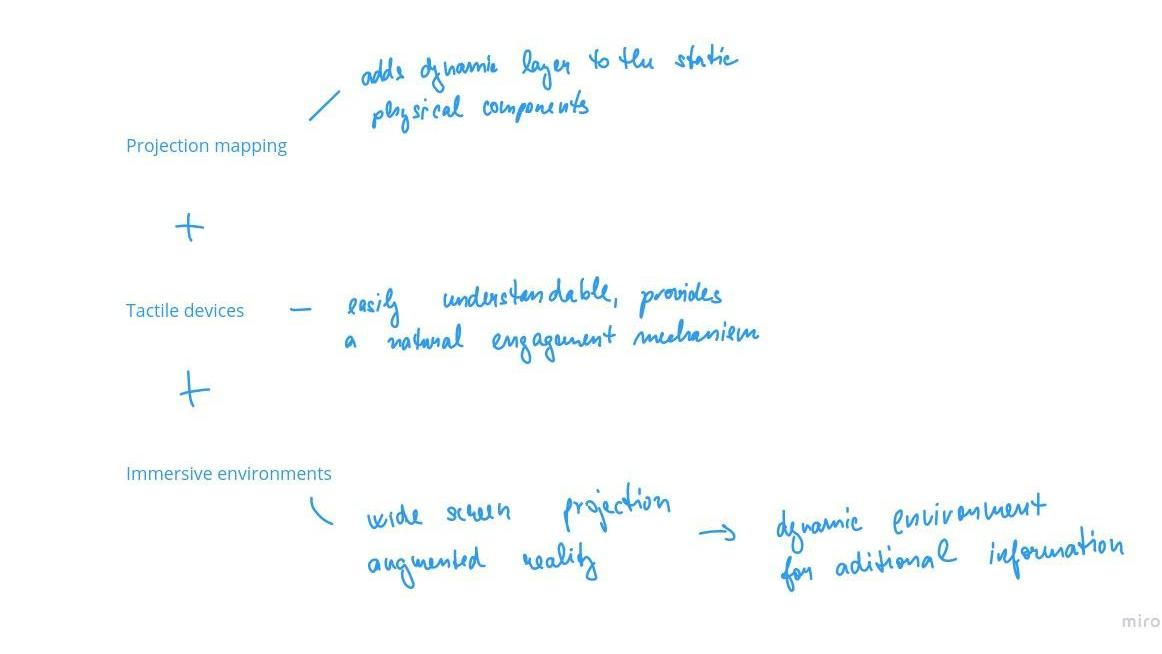
\includegraphics[width=\linewidth]{img/medium.jpg}
    \caption{Presentation medium - notes}
\end{figure}

\subsection{Applications}

There already is a range of available software solutions for urban data visualization. Here is a list of some of them:

\paragraph{ArcGis} 
Esri offers a range of GIS products under the name of ArcGIS. It is a full suite of software for geospatial visualization and analysis. ArcGIS Urban focuses on urban data, visualization, and planning. It is a web-based application. As it is commercial software with full-time support, it is a widely popular solution used by local authorities. ArcGis supports a wide range of proprietary formats (namely ArcIMS, DGN, DWG, DXF, and a range of raster formats). 

\paragraph{QGIS} An open-source tool for creating, viewing, and editing geospatial information. Supports a wide range of formats (Esri Shapefiles, ArcInfo files, MapInfo files, .csv, OpenStreetMap data, PostGis data together with a group of database-based file formats). There is a QGIS plugin, Qgis2threejs, which provides a way to view 3D content, but it appears that the only supported input format is .hgt - DEM (Digital elevation model) format. From version 3.0, there is built-in support for 3D content; supported formats are mostly Esri Shapefiles and raster formats (e.g., GeoTiff). It is possible to export static images as well as short animations created from time-series data. The current capabilities of the program limit the styling options. 

\paragraph{kepler.gl}
Kepler.gl is an open-source visualization application developed by vis.gl. The tool was created and popularized in collaboration with UBER; the main focus is scalability and good performance. The tool is based on Deck.gl, also made by vis.gl, a WebGL-based rendering framework optimized for big data visualizations. The application uses a concept of layers and filters for displaying the imported data. Each layer is an isolated entity with its own base geometry (lines, arcs, points, hex or rectangular grid, heatmap, etc.) and style. 
The application uses OpenStreetMap and Mapbox data as a source for 2D maps and 3D models of buildings. The only missing 3D component is the terrain height. It is possible to use Kepler.gl as a Python library for visualization inside Jupyter Notebooks. The supported formats include CSV, GeoJSON, and proprietary JSON-based application format. 

\paragraph{Movement}
This application was also developed by vis.gl in collaboration with UBER. The primary focus of this application the visualization of transport-related data. This project stands on the border of visualization and data analysis. Unlike the previous solutions, this application was developed to present a fixed set of curated datasets. The goal is to help cities (they operate only in a limited number of cities) to reduce congestion, emissions, and improve road safety.\\

\paragraph{Cesium}
Cesium is a platform for building geospatial applications. They provide a way to push 3D content to both web (CesiumJS) and Unreal Engine. A part of their services is a platform called Ion, which automatically tiles and optimizes the content for both web and the game engine and offers a library of assets such as images, terrain, and building models. Cesium offers a free plan with a limited amount of data. However, the platform is targeted towards commercial projects and offers pre-paid plans with higher bandwidth.\\


\subsection{Frameworks}
In terms of visualization frameworks, there are several existing solutions. There is a slight difference between the previous examples and these frameworks - the frameworks are not standalone visualization solutions. The visualization frameworks usually provide a set of features (data management, rendering, etc.) used throughout the visualization pipeline. 

\paragraph{3DCityDB}
3DCityDB is a framework oriented towards effective storing, analysis, and export of the urban data. Part of the toolkit is also a visualization client, but the framework is mainly oriented towards data management. The idea behind this framework is the use of the CityGML standard as the base scheme for the data representation. The framework supports export into several formats, such as Collada, glTF, and KML.

\paragraph{Vis.gl Frameworks}
Vis.gl develops several web-based frameworks for visualization. Deck.gl is a WebGL-based rendering framework for visual exploratory data analysis of large geospatial datasets. It's built to be compatible with React (app flow and UI) and Mapbox (source of the base map). A more general-purpose visualization framework is Luma.gl, also a WebGL-based toolkit. To provide a way for plotting various data in 2D, vis.gl developed a library React-vis. As the name already suggests, it is built to be compatible with the React app model.

\paragraph{Blender GIS and Up3date}
Several plugins allow for the import of GIS data into Blender, namely Blender GIS or Up3date, which are both still maintained. The supported files include CityJSON, Shapefile vector, raster image, GeoTIFF DEM, OpenStreetMap. 

\paragraph{Game Engines}
TODO

\begin{figure}[h]
    \centering
    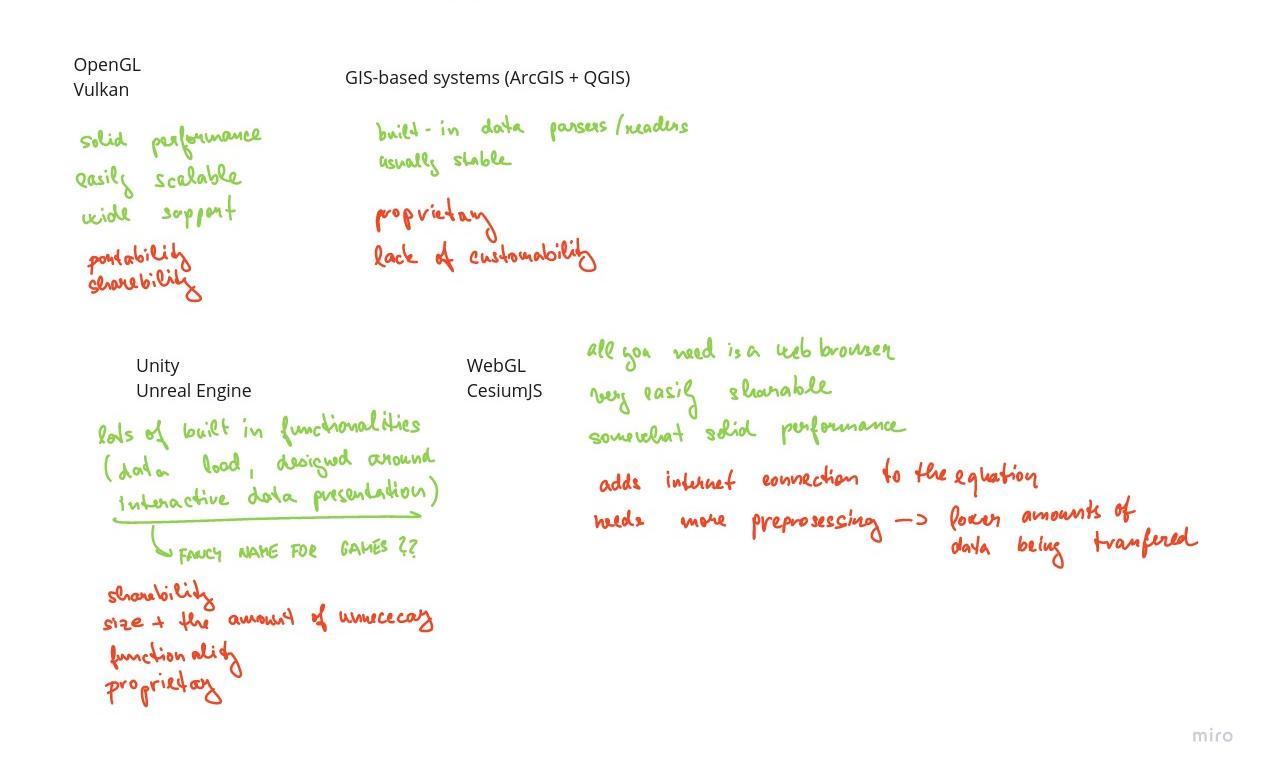
\includegraphics[width=\linewidth]{img/frameworknotes.jpg}
    \caption{Frameworks - notes}
\end{figure}